\documentclass[11pt]{article}
\usepackage{listings}
\usepackage{xcolor}
\usepackage{graphicx}
\usepackage{csquotes}
\usepackage{amsmath}
\usepackage{url}
\usepackage[english]{babel} % Valid line breaking
 
\definecolor{codegreen}{rgb}{0,0.6,0}
\definecolor{codegray}{rgb}{0.5,0.5,0.5}
\definecolor{codepurple}{rgb}{0.58,0,0.82}
\definecolor{backcolour}{rgb}{0.95,0.95,0.92}
 
\lstdefinestyle{JavaStyle}{
    backgroundcolor=\color{backcolour},   
    commentstyle=\color{codegreen},
    keywordstyle=\color{magenta},
    numberstyle=\tiny\color{codegray},
    stringstyle=\color{codepurple},
    basicstyle=\ttfamily\footnotesize,
    breakatwhitespace=false,         
    breaklines=true,                 
    captionpos=b,                    
    keepspaces=true,                 
    numbers=left,                    
    numbersep=5pt,                  
    showspaces=false,                
    showstringspaces=false,
    showtabs=false,                  
    tabsize=2
}
 
\lstset{style=JavaStyle}

\renewcommand{\today}{\ifcase \month \or January\or February\or March\or April\or May\or June\or July\or August\or September\or October\or November\or December\fi, \number \year} 
\newcommand{\topic}{Project Lucene}
\newcommand{\paper}{StackOverflow\\
	\small{\textit{M INF \  2019-2020}}
}
\newcommand{\team}{
	\=Johannes Akkermans, \\\>Randy Paredis
}

\begin{document}
\title{\textmd{\textbf{Information Retrieval}}\\\normalsize\vspace{0.1in}\Large{\topic}\\\large{\paper}\Large\\\vspace{0.1in}}
\author{}
\date{\today}
\maketitle
\begin{center}
	\parbox{0cm}{
		\begin{tabbing}
		\textbf{Group:} \team
		\end{tabbing}
	}
\end{center}

\vspace*{1em}

\begin{abstract}
    Lucene is a powerful Java-tool that allows for easy information retrieval of large datasets. The goal of this project was to apply Lucene on the StackOverflow data and study its feasability. Additionally, we will try to improve the overall performance of the retrieval by applying some techniques we've seen in class.
\end{abstract}

\newpage

% Study the feasibility of using Lucene to add retrieval capabilities to the StackOverflow repository provided to you. Describe the functionality offered by Lucene, such as the types of indices that are included, the different score models, etc. How does Lucene store the index, does it have spell correction? Include a benchmarking study of the performance of the retrieval performance. Manually label some documents. One acceptable approach is to use the titles of the questions as the query, and only index the remaining parts of the documents. In this way a ground truth can be generated rather easily. This first part is expected to be about 10 pages.

\section{Lucene}\label{sec:lucene}
Apache Lucene is a free and open-source search engine software library written in Java. It allows for full-text indexing and searching making it a perfect fit for the project at hand. \cite{lucene-wiki}

There are a lot of features Lucene offers, but we will not need all of them. This is why we will gradually go over our project and the Lucene features we've used to obtain the described results. All specific details on the internal workings of Lucene are described in its documentation, publicly available on \cite{lucene}.

\subsection{Dataset}
Of course, before we can do anything, we require a dataset on which we will execute Lucene. In order to do that, we've downloaded the massive dataset from StackOverflow\footnote{From the website indicated in the assignment.}. Next, we extracted this dataset before running a Python script that parses this massive xml-file into $2\,010\,607$ smaller files, containing questions and answers, all of whom had \texttt{python} or \texttt{c++} in its tags. Every 1000 files are put into a sub-folder, making sure our operating systems can handle this amount of data. The overall size approximates 7 gigabytes, which is why it's not accompanied with our submission of the project.

Now that we have this dataset, we can start looking at Lucene.

\subsection{Analyzer and Setup}\label{sec:analysetup}
The first and foremost thing to do in Lucene is to create an \texttt{Analyzer}. As the name might suggest, it will analyze text by building \texttt{TokenStreams}\footnote{\texttt{org.apache.lucene.analysis.TokenStream}}. More theoretically, it describes a policy on how items are extracted from text.

Lucene comes with a \texttt{StandardAnalyzer} class\footnote{\texttt{org.apache.lucene.analysis.standard.StandardAnalyzer}}. This subclass of the abstract \texttt{Analyzer} has a very broad use case, seeing as it correctly splits unicode text, turns everything to lowercase and removes a set of English stop words. It can be created quite easily:
\begin{lstlisting}[language=Java]
StandardAnalyzer analyzer = new StandardAnalyzer();
\end{lstlisting}

Alas, the \texttt{StandardAnalyzer} does not take into account that our data consists of a lot of xml-files. On top of that, xml makes use of a special character encoding system that does not map straightforwardly on unicode. This is an issue we need to keep in mind when processing our data. Luckily, there is the possibility of creating a custom \texttt{Analyzer} (in our project, this is the \texttt{MyCustomAnalyzer} class) to solve this issue. More on the \texttt{MyCustomAnalyzer} in section \ref{sec:optimizations}.

\subsection{Indexing}\label{sec:indexing}
\subsubsection{Index Directory}
Now that we have an \texttt{Analyzer}, we need a place to keep track of the indexing. Because indexing itself is an expensive operation, it will not be done before every search and, on top of that, it will be stored in a folder on disk, making sure your indexes remain consistent (and above all: existent) between multiple executions.

In our implementation, we create a new directory, called \texttt{.search} in which we will store this information. If this directory already exists, it is cleared beforehand. Note that, this way, we will bypass the usecase of storing these files in a directory.
\begin{lstlisting}[language=Java]
Directory index = new MMapDirectory(Paths.get(".search"));
\end{lstlisting}

\subsubsection{Indexing of Files}\label{sec:indexfiles}
The dataset we've used was too big to index as a whole for the scope of our project. This is why our code only indexes on a part of this data ($10\,000$ files), which was randomly selected using Java's builtin random number generator with a fixed seed of 420 (for repeatability).

In order to do so, we had to flatten our dataset in such a way that our OS could handle it. Here is where we discovered a problem on MacOS (compared to Ubuntu LTS 18.04, that is). On Mac, the \texttt{File} class actually opens the file, causing this to be a costly operation. We solved this inconvenience via iterating over the filenames and only taking those ending in ``xml''\footnote{This method has as a downside that it will not work on Windows systems. Mainly because we hardcoded the ``\texttt{/}'' as a path separator.}.

Either way, after we've obtained our files to index, we will add all these documents to an \texttt{IndexWriter}\footnote{\texttt{org.apache.lucene.index.IndexWriter}}. This object basically keeps track of all labeled information of the documents in our dataset.
\begin{lstlisting}[language=Java]
IndexWriterConfig config = new IndexWriterConfig(analyzer);
IndexWriter w = new IndexWriter(index, config);
\end{lstlisting}

For the purpose of the assignment, we indexed the fields \textit{name} (i.e. the filename), \textit{title}, \textit{body}, \textit{tags} and \textit{answers}. These last four need to be transformed in such a way that all special characters and capitalization are removed (as mentioned in section \ref{sec:analysetup}, see also section \ref{sec:query}). This is done by our \texttt{MyCustomAnalyzer} (as will be discussed in section \ref{sec:optimizations}). Additionally, the \textit{answers} are all joined together, separated with two newline characters (\texttt{\textbackslash n}), for ease of use.

Internally, Lucene does not search all the files, because that would be too costly. In fact, this indexing stage creates a list of indexes and the pages they refer to, similarly to something you might see in a handbook. These indexes are called ``\textit{reverse indexes}''. \cite{lucene-tutorial}

\subsubsection{Storing the Feature Vectors}\label{sec:fv}
Because we will need it later on (see section \ref{sec:rocchio}), we will also tell Lucene it needs to store the term vectors of all fields. This way, we hope to be able to use the Vector Space Model (VSM) Lucene uses behind the scenes.

\subsubsection{Index File Formats}
As mentioned before, Lucene stores the indexing data in a set of files. Its contents are not entirely readable by a human\footnote{Using ourselves as a point of reference.}, making us suspect there is some sort compression or encoding that's being done by Lucene. Our suspicions were confirmed in \cite{lucene}, which also gives an extended overview of this encoding.

\subsection{Score Models}
There are numerous scoring models bundled with Lucene (as we will discuss in section \ref{sec:scmodels}). By default, Lucene uses the \texttt{TFIDFSimilarity}\footnote{\texttt{org.apache.lucene.search.similarities.TFIDFSimilarity}}.

The fastest way to obtain a score in Lucene, would by via the following code:
\begin{lstlisting}[language=Java]
// Search with the query
IndexReader reader = DirectoryReader.open(index);
IndexSearcher searcher = new IndexSearcher(reader);
TopDocs docs = searcher.search(q, cnt);
ScoreDoc[] hits = docs.scoreDocs;
\end{lstlisting}

Here, we would search for a query \texttt{q} and return at most \texttt{cnt} documents that match it, ordered by highest score first. To quote scoring in the words from \cite{lucene}, which also describes our love-hate relationship with it:
\begin{displayquote}
    \textsl{Lucene scoring is the heart of why we all love Lucene. It is blazingly fast and it hides almost all of the complexity from the user. In a nutshell, it works. At least, that is, until it doesn't work, or doesn't work as one would expect it to work.}
\end{displayquote}

Allow us to emphasize that this quote comes unedited from their own website, basically stating that Lucene does not always works the way you want it to work, an issue we have experienced on numerous occasions during this project (especially in section \ref{sec:rocchio}).

\subsubsection{Similarity Scoring}\label{sec:ss}
From \cite{lucene}, we can also conclude how its scoring actually works internally. From the course, we know there must be some similarity checking formula at work. We find that Lucene makes use of the \textsf{VSM score}, better known as the \textsf{cosine simularity} (with $V(q)$ and $V(d)$ weighed query vectors):
$$cosine\_similarity(q, d) = \frac{V(q)\cdot V(d)}{\vert V(q)\vert\cdot\vert V(d)\vert}$$
Its scoring formula therefore becomes:
\begin{align*}
    score(q, d) =&\ coord(q, d)\cdot queryNorm(q)\ \cdot\\
    &\sum_{t \in q}\left[tf(t\in d)\cdot idf(t)^2 \cdot t.getBoost()\cdot norm(t, d)\right]
\end{align*}

\section{Query Building}\label{sec:query}
Even though Lucene makes use of a Vector Space Model (VSM), it is by default completely hidden. On top of that, we haven't found any information (nor in the documentation, nor anywhere online) on how to search the dataset by vector. We would have to create our own scoring system, an idea we quickly discarded because of the massive size of our data\footnote{We also discarded this idea because we did not believe this was intended with the assignment. In fact, the fast and efficient workings of the similarity checking as described in section \ref{sec:ss} was a major influence in this decision.}. Instead, we decided to use the builtin binary query system, which is tested and optimized for searching\footnote{On top of that, it is impossible to obtain the VSM without giving such a query string.}.

To allow for simple manipulations of the queries we introduced the notion of a \texttt{QueryBuilder}. Based on a string with the valid search criteria, we create a query that follows the Lucene query syntax and remains conform with the inputted data. Even though this may seem as an unnecessary additional parsing step, it will become useful later on.

Let's take a deeper dive into our \texttt{QueryBuilder}.

\subsection{String Replacements}
Before we even start to build our query, we need to transform a string into a general syntax that can be easily understood without too much issues. We identify three phases:

First we have the \textsf{trimming phase}. Here, we remove all whitespace surrounding our query, i.e. at the beginning and the end. Although the Lucene documentation does not explicitly state this as a requirement, we wanted to make sure it does not cause any undefined behaviour.

Next, we transform our string into lowercase format. Let's call this the \textsf{lowercase transformation phase}. This was done because matching on capitalization is not useful within our problem domain. Of course, this also requires our documents to be transformed in a similar manner (see sections \ref{sec:indexing} and \ref{sec:optimizations}).

Finally, there is the \textsf{alphanumerisation phase}\footnote{Or that's at least how we called it.}. Here, we will remove all special characters from our queries, seeing as they will only cause issues and strange behaviour (i.e. leaving a period in the query could result in the match of any character). Admittedly, in doing so we loose the ability to match hyphenated words and other special cases like the query ``\texttt{c++}''. It was our hypothesis that these words would not take up too much of the language and thus are irrelevant in this context.

Assuming our query is stored in the variable \texttt{word}, these three phases look, quite elegantly, like this:
\begin{lstlisting}[language=Java]
word.strip().toLowerCase().replaceAll("[^a-z0-9 ]", "")
\end{lstlisting}

Note that this only applies for the query itself. As will be discussed in section \ref{sec:optimizations}, for the documents themselves, this will be achieved via applying some additional filters to the analyzer.

\subsection{String Separation}
As you might have guessed from the previous section, we have only removed all whitespace from the beginning and the end of our string. All spaces in the middle are left and for good reason. They tell our system that all of those words \textbf{must} appear together.

If we look at Google and how they go about spaces, you might be able to deduce from the url, that they replace all spaces with an \texttt{AND}-gate (the plus sign). This not only allows words to be in a different word order, but also allows words not to be next to one another. This method works wonders for Google, so why wouldn't it be in our system?

Let's say we have the query ``\texttt{python database setup}''. By default, Lucene adds an \texttt{OR}-gate between these terms, but we want to enforce that these three words occur together (not necessarily in that order, or next to one another). Thus, we will add explicit \texttt{AND}-gates between them. Therefore, we obtain the query ``\texttt{python AND database AND setup}'' as an input to Lucene.

For the further query building, we will be looking at this list of whitespace-less strings, separated with an \texttt{AND}. Such an individual string will be referred to as a ``\textit{term}''.
\begin{lstlisting}[language=Java]
String[] terms = word.split(" ");
String newWord = String.join(" AND ", terms);
\end{lstlisting}

\subsection{Spell Correction}
Fuzzy search is a powerful tool. It allows a search engine to find words that are similar, just in case the user made a typo in the query. Fuzzy search can be referred to as ``\textit{Did You Mean...?}'' functionality.

In Lucene no spell checking is used by default, but there are multiple ways to obtain fuzzy search.
\begin{itemize}
    \item Use the Lucene query syntax for fuzzy search. This is done via adding the tilde ($\sim$) to the back of a term. In exploring how Lucene works and what influence this syntax had, we have found it does not fully accomplish what we want to achieve.\\
    By default, this syntax will allow words to be at most 50\% different. Within this context, the word ``\texttt{bear}'' will also match ``\texttt{beer}'', ``\texttt{boar}'', ``\texttt{bend}'', ``\texttt{fear}'', ``\texttt{feat}'', ``\texttt{rear}'' and ``\texttt{zeal}'' to name a few. All of the words mentioned above are real words, but the similarity measure does not make that assumption. Words like ``\texttt{glar}'', ``\texttt{qeaq}'' and ``\texttt{eeaa}'' does not exist in the English language, but will also be matched. Hypothetically, a set of documents on a fictional alien language might use these non-existing words a lot. If there are very few documents describing bears in the dataset, I might get a lot of fictional alien language information, while I did not want this.
    \item Use Lucene wildcards. While at first sight, this might be a good idea, on second thought there are way too many issues with this method. First, a term is not allowed to start with a wildcard (presumably because it would make it left-recursive). Secondly, there are way too many possible locations to add wildcards. Do you add them between all letters? Do you replace all letters? Do you do a combination of the two? For this combination method and an $n$-letter word, there are $2^{2(n - 1)}$ possibilities for adding wildcards.\\
    For instance, in a 5-letter word ``\texttt{abcde}'', wildcards can be located at the letter locations (except for the \texttt{a}), or between all letters, giving us $2^{4+4} = 2^{2(5-1)} = 2^8 = 256$ possibilities.
    \item Generate all possible replacements for a term. We have an alphabet of 26 letters and 10 different digits with whom we can replace every single letter. But we hit the same wall as with the wildcards, only with a much higher set of possibilities ($36^{n}$ instead of $2^{2n-1}$). Figure \ref{fig:wa} shows that, no matter the value of $n$, this option will always yield more possibilities.
    \begin{figure}[h!]
        \centering
        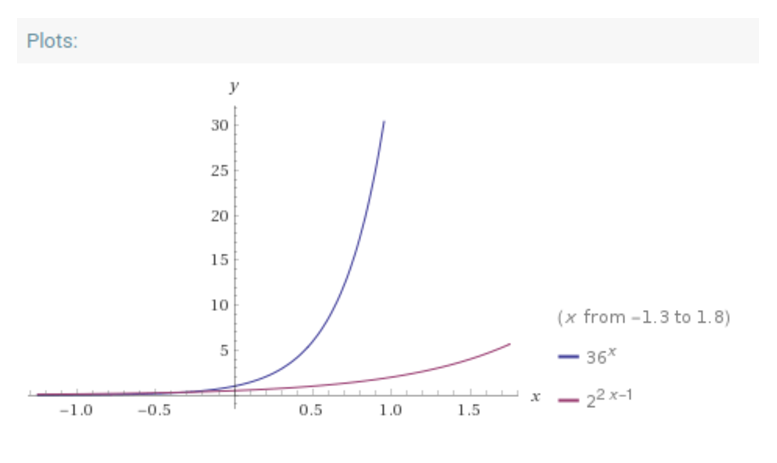
\includegraphics[width=.75\textwidth]{images/plots.eps}
        \caption{WolframAlpha-made plot of both $y=36^{x}$ and $y=2^{2x-1}$.}
        \label{fig:wa}
    \end{figure}\\
    On top of that, if we say that we only replace one or two letters at a time, there are still unexplored options. Let's say we want to look for ``\texttt{code}'', but accidentally only type ``\texttt{cod}'', this method will not find the right documents.
    \item Lucene has this \texttt{SpellChecker} class that can suggest the $n$ closest words in the dictionary of all files. This method allows us to resolve typos and tweak the amount of possible replacements\footnote{It's illogical that each word should match all of its possibilities. From ``\texttt{bear}'' to ``\texttt{beard}'', ``\texttt{boar}'' or ``\texttt{beer}'' are smaller changes than replacing it with ``\texttt{glad}''.}. For our purposes, we assumed 5 similar words (and the current one, making it 6 checks) should do the trick. We merge them all together in one big \texttt{OR}-gate for each term.
\end{itemize}
As you can guess, we have decided on the latter option, which can be implemented as follows (assume \texttt{term} is our term):
\begin{lstlisting}[language=Java]
// Did you mean? https://www.javacodegeeks.com/2010/05/did-you-mean-feature-lucene-spell.html
SpellChecker spellchecker = new SpellChecker(spellIndexDirectory);
// To index a field of a user index:
spellchecker.indexDictionary(new LuceneDictionary(my_lucene_reader, a_field));
// To index a file containing words:
spellchecker.indexDictionary(new PlainTextDictionary(
    new File("myfile.txt")));
String[] suggestions = spellchecker.suggestSimilar(term, 5);
String newTerm = "(" + String.join(" OR ", suggestions) + ")";
\end{lstlisting}
% https://lucene.apache.org/core/6_0_1/suggest/org/apache/lucene/search/spell/SpellChecker.html
% Mss: https://www.inetsoftware.de/documentation/other-products/jortho/apispec/

Combined with \textsf{String Separation}, we get:
\begin{lstlisting}[language=Java]
SpellChecker spellchecker = new SpellChecker(spellIndexDirectory);
spellchecker.indexDictionary(new LuceneDictionary(my_lucene_reader, a_field));
spellchecker.indexDictionary(new PlainTextDictionary(
    new File("myfile.txt")));
String[] terms = word.split(" ");
ArrayList<String> newTerms = new ArrayList<>();
for(String term: terms) {
    // Just in case there are multiple spaces
    if(term.isEmpty()) { continue; }
    
    List<String> suggestions = new ArrayList<>(Arrays.asList(spellchecker.suggestSimilar(term, 5));
    
    // Make sure the actual term is part of the query
    if(!suggestions.contains(term)) {
        suggestions.add(term);
    }
    newTerms.add("(" + String.join(" OR ", suggestions) + ")")
}
String newWord = String.join(" AND ", newTerms);
\end{lstlisting}

\section{Benchmark Study}\label{sec:bstudy}
To evaluate the retrieval performance of Lucene, the PR- and the ROC-curve will do great at visualizing this performance. To plot these curves, the Precision ($P$), Recall ($R = TPR$) and Fallout ($F = FPR$) need to be computed, which will be realized by \textit{manual labeling}. Formulas for these numbers are given as follows:
\begin{align*}
    P &= \frac{TP}{TP+FP}&
    R &= \frac{TP}{TP+FN}&
    F &= \frac{FP}{FP+TN}
\end{align*}

\subsection{Manual Labeling}
Contrary to what it's name might suggest, we did not select a number of documents which we labeled by hand for a specific query. This seemed to bring us too far away from the project scope and therefore we focused on finding an acceptable algorithm to solve this issue. We were mainly inspired by this part of the assignment:

\begin{displayquote}
    \textsl{One acceptable approach is to use the titles of the questions as the query, and only index the remaining parts of the documents. In this way a ground truth can be generated rather easily.}
\end{displayquote}

We tried different methods for achieving our goal and, at long last, we stranded on the method described below.

First things first, we have a system that can determine the score of all documents, given a set of queries. Unfortunately, this system alone is not enough in determining the amount of True Positives ($TP$), False Negatives ($FN$), False Positives ($FP$) and True Negatives ($TN$). We need a way to consistently label documents as either ``\textit{correct}'' or ``\textit{incorrect}''. And this can be done by exploiting the use of \textit{tags}.

\subsubsection{Tags as Queries}
Each question in our dataset has a group of \textit{tags} associated to it. These \textit{tags} generally mark the topics or problem domains to which the questions apply, therefore we can state that, if we search for any group of tags, all documents that have these tags can be marked as ``\textit{correct}''.

For instance, a question that concerns ``\texttt{efficient string comparison in python}'', with tags ``\texttt{string-comparison}'' and ``\texttt{python}'' must be a document that is returned when looking for ``\texttt{python}'', ``\texttt{string-comparison}'', or ``\texttt{python string-comparison}''\footnote{Please denote that ``\texttt{string-comparison}'' is used as a tag for readability of this report, but internally, in our code, this is one of the tags we won't process (see further).}.

Now, how do we go about doing this? On indexing time, we will keep some sort of a query cache\footnote{It is slightly more efficient to do this at indexing time, but it is perfectly doable to do this afterwards, in the actual performance checking.}. This cache is a list of strings that we can use as queries for benchmark purposes. For every question we have in our dataset, we create a new entry in this cache, concerning all unique possible combinations of the set of \textit{tags} for this question. For instance, the tags ``\texttt{python}'', ``\texttt{c}'' and ``\texttt{java}'' become the entries \{``\texttt{c}'', ``\texttt{java}'', ``\texttt{python}'', ``\texttt{c python}'', ``\texttt{java python}'', ``\texttt{c java}'', ``\texttt{c java python}''\} (notice the alphabetical ordering).

Because we know there are a lot of queries that will be created with this method, we will not concern ourselves with tags that contain anything but alphabetical characters and discard those entries entirely.

Of course, this also implies that we will remove the \textit{tags} from the fields we search on, because this would not make too much sense\footnote{Some experimentation has shown that, in practice, this is not necessary, because the results will be roughly the same.}.

\subsection{Performance Scoring}
And then comes the scoring phase. For all of these queries, we will determine both the scores and its relevance of all documents as discussed above. This gives us two general information files.

The first one is a results file that states for each question how good it performed on which queries. Secondly, there is a relevance file where each query maps to a list of question ids. These ids represent the questions that were marks ``\textit{correct}'' for the corresponding query.

A \textsf{Hapax Legomenon} (or a \textsf{hapax} for short) is a word or a concept that only occurs only once in a given context (see \cite{hapax}). Within our context, we can state that a \textit{tag} is a \textsf{hapax} if there is only one document that uses it. Or, in layman's terms, a \textit{tag} (or a set thereof) that is only used by a single question. These do not give an accurate representation of our dataset, so we remove them on the whole. Similarly, we believe that a \textit{tag} that's only used by two questions does not provide enough information for our data.

From the $20\,710$ different \textit{tag} combinations that were used as queries, we will only look at the $2\,099$ queries that were able to mark more than two questions as being ``\textit{correct}''.

\subsubsection{PR and ROC}
For each query in this set of $2\,099$ unique \textit{tag} combinations, we can now determine the top-$k$ precision, recall and fallout (as is shown in the lecture slides), which allows us to create the Precision-Recall (PR) Curve and the ROC-Curve for each query.

Because this will yield a lot of curves, most of which without any significant features, we have decided to represent the PR and ROC as an upper bound (i.e. the curve that is generally higher than all values). Note that this may give a skewed view of our results, but it seemed the most doable option. We tried using (weighed) averages, minimals, differences..., but unfortunately all of these resulted in plots with strange artifacts. An example of such a plot is shown in figure \ref{fig:artifact}.

\begin{figure}[htp]
	\centering
	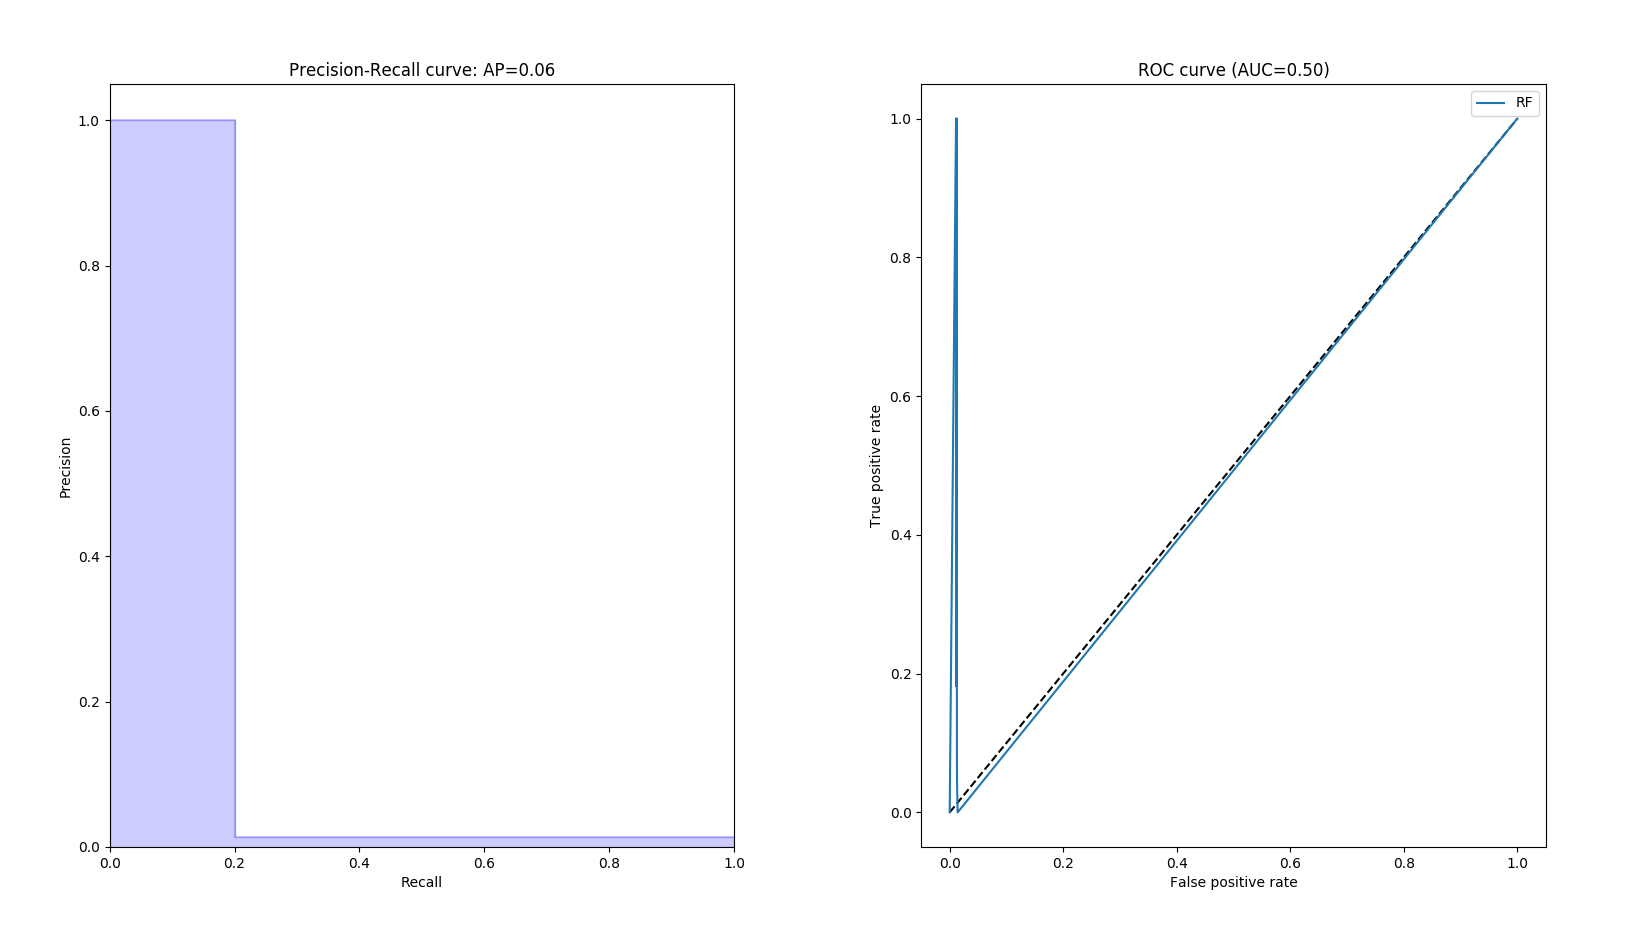
\includegraphics[width=\textwidth]{images/artifact}
	\caption{PR/ROC plots with artifacts due to maximization}
	\label{fig:artifact}
\end{figure}

\subsubsection{Initial Score}
Using the \texttt{StandardAnalyzer} of Lucene\footnote{Which does a lot behind the scenes, including (but not limited to) removing stopwords and lowercase transformations}, the scores are computed as described above. This gives us an idea how well Lucene initially performs.

Using the averaged PR- and ROC-curves to visualize the results, we can conclude from Figure \ref{fig:initBP}, Lucene is doing an ok job for the task at hand, but nothing spectacular.

\begin{figure}[htp]
    \centering
    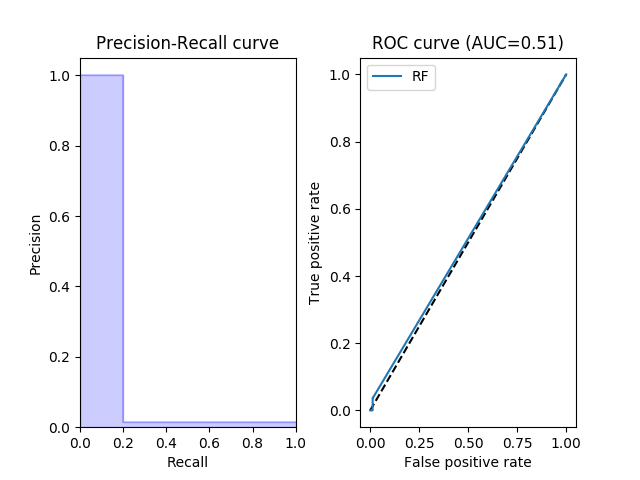
\includegraphics[width=\textwidth]{images/StandardAnalyzer}
    \caption{Results initial Benchmark Performance.}
    \label{fig:initBP}
\end{figure}

\subsection{Scoring Models}\label{sec:scmodels}
To check whether the scoring models have any influence on the performance, the different \texttt{Similarity} measures have been used: \texttt{TFIDFSimilarity}\footnote{\texttt{org.apache.lucene.search.similarities.TFIDFSimilarity}} and \texttt{BooleanSimilarity}\footnote{\texttt{org.apache.lucene.search.similarities.BooleanSimilarity}}. 

Different similarity measurements have an impact on the performance of the system. Figure \ref{fig:bool} gives an overview of the boolean similairty where the terms score is equal to their query boost. The other measurement is the Tf-Idf similiartity; this scores the documents based on the cosine similarity in a VSM as described in section \ref{sec:ss}. The Tf-Idf have much better performance results, that's why we will use the scoring model Tf-Idf for analyzing the documents.

\begin{figure}[htp]
	\centering
	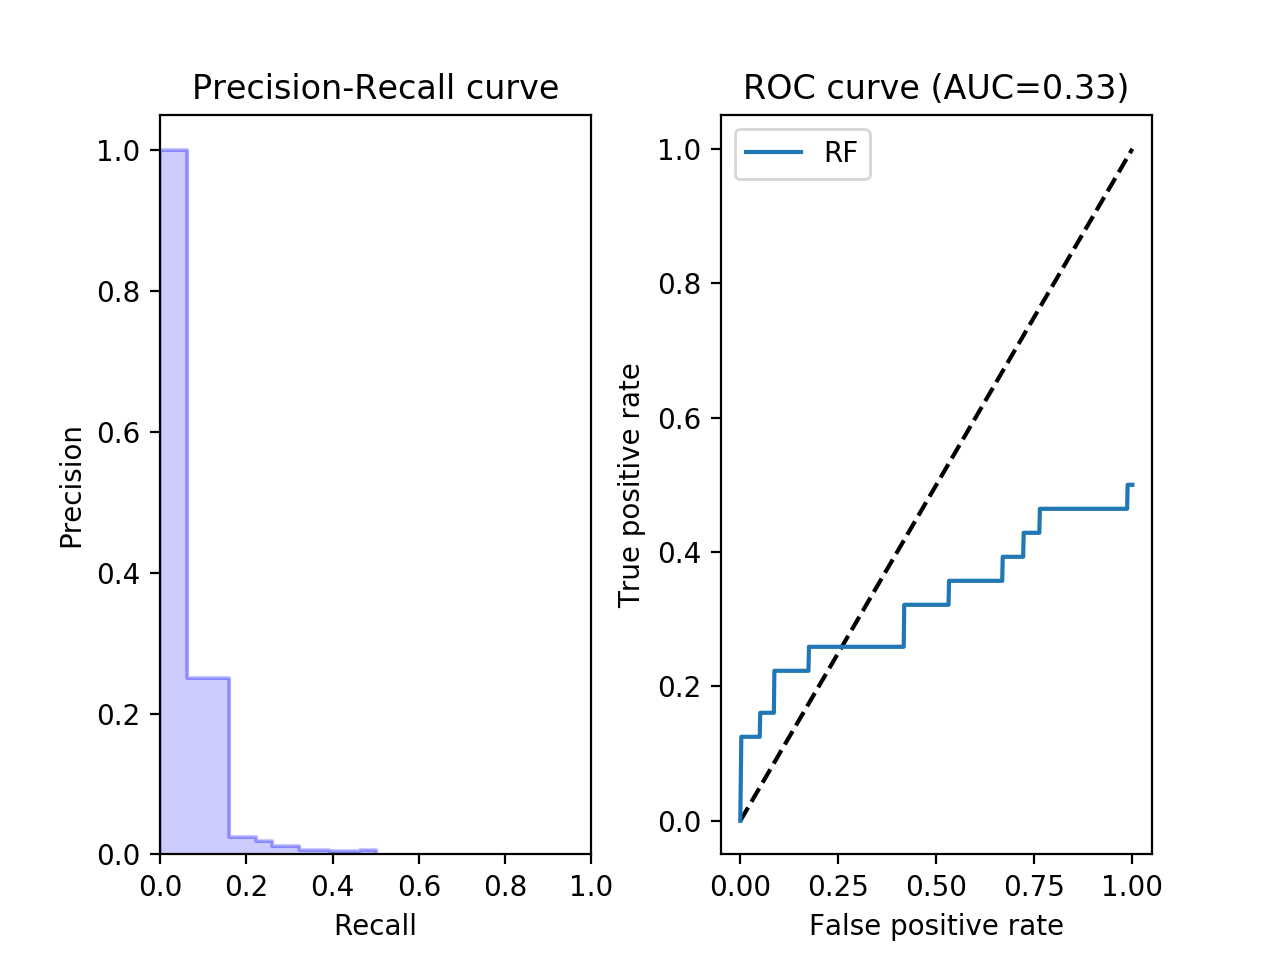
\includegraphics[width=\textwidth]{images/Boolean-Standard}
	\caption{An overview of the standard Analyzer using a Boolean Similarity measurement}
	\label{fig:bool}
\end{figure}
\begin{figure}[htp]
	\centering
	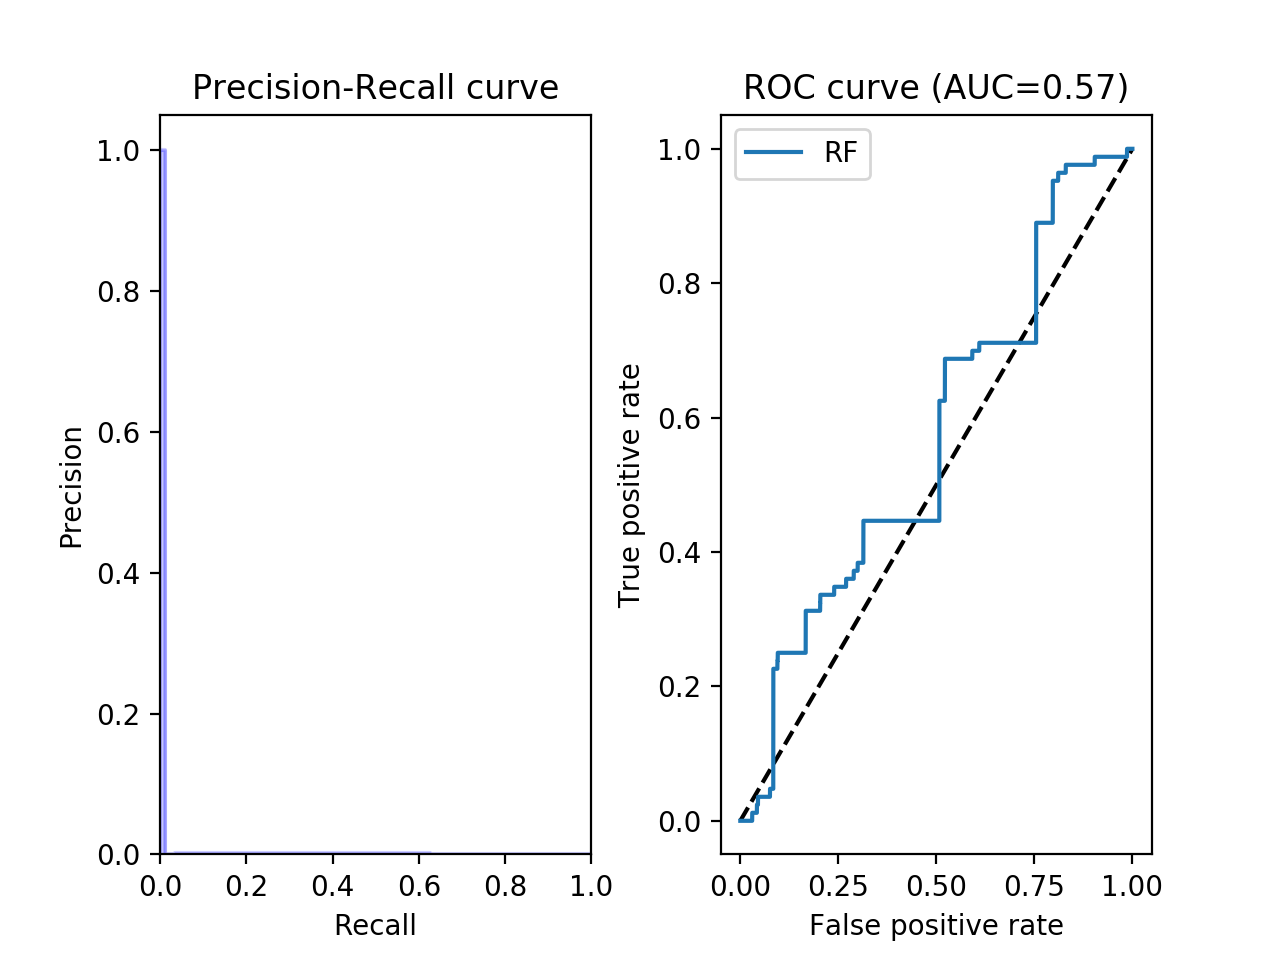
\includegraphics[width=\textwidth]{images/Tfidf-standard}
	\caption{An overview of the standard Analyzer using a Tf-Idf Similarity measurement}
	\label{fig:tfidf}
\end{figure}

\section{Optimizations}\label{sec:optimizations}
As was clear from figure \ref{fig:initBP}, we can do better. This is why we will try to optimize our algorithms, in the hope of obtaining better results. In order to achieve this goal, we will reimplement the \texttt{StandardAnalyzer} as a basis for our \texttt{MyCustomAnalyzer} and work from there.

\subsection{Removing Special Characters and Whitespace}
As discussed in depth in section \ref{sec:query}, we will transform our fields so all specialities are discarded. If we base ourselves on the \texttt{StandardAnalyzer} and on the transformations we want to apply, as per section \ref{sec:query}, all that's left to do in order to have a valid transformation is to remove all non-alphanumerical characters and additional whitespace from our text.

This is done via adding a \texttt{PatternReplaceFilter}\footnote{\texttt{org.apache.lucene.analysis.pattern.PatternReplaceFilter}} and a \texttt{TrimFilter}\footnote{\texttt{org.apache.lucene.analysis.miscellaneous.TrimFilter}} in our \texttt{Analyzer}.

In figure \ref{fig:alphanumeric}, you can find that there was no significant difference compared to the original plot.
\begin{figure}[htp]
    \centering
    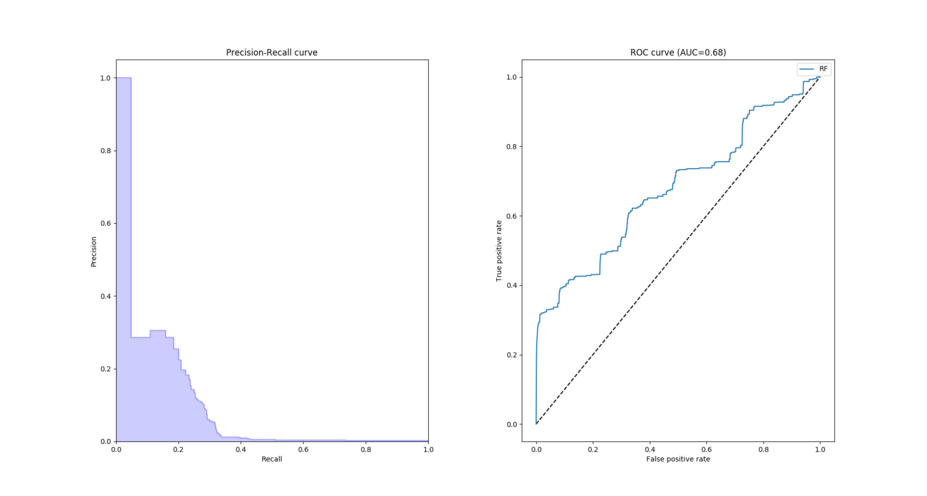
\includegraphics[width=\textwidth]{images/customAna-trim}
    \caption{Results Benchmark Performance with Initial Filters.}
    \label{fig:alphanumeric}
\end{figure}

\subsubsection{Word Delimiter}\label{sec:word-delimiter}
The \texttt{StandardTokenizer} will be extended with a \texttt{WordDelimiterGraphFilter}\footnote{\texttt{org.apache.lucene.analysis.miscellaneous.WordDelimiterGraphFilter}}. This will split the words into multiple subwords and performs optional transformations on subword groups. \cite{lucene}

For example, if someone wants to search for ``\texttt{Macbook}'', but the user types ``\texttt{Mac Book}''. The WordDelimiter will catch this query because the word ``\texttt{Macbook}'' will internally saved as \{``\texttt{Mac}'', ``\texttt{Book}'', ``\texttt{Macbook}''\}. This way, we can cope with different cases of compound words.

At first, it sounds like a good idea, but, unfortunately, it doesn't have a huge impact on the performance. It even results in the same PR- and ROC-cuves as Figure \ref{fig:alphanumeric}! We believe this is because this kind of filter does not apply for our current set of queries.

\subsubsection{Stemming}\label{sec:stemming}
Next, stemming\footnote{\texttt{org.apache.lucene.analysis.PorterStemFilter}} has been added to the analyzer such that multiple variants of a word are mapped to the same word (i.e. plurals are mapped to its singular). Strangely enough, there is no performance increase on this front, as you may be able to deduce from figure \ref{fig:stemming}. (Yes, it looks once more like the very same plot, possibly because of the way we generate the plots.)

\begin{figure}[htp]
    \centering
    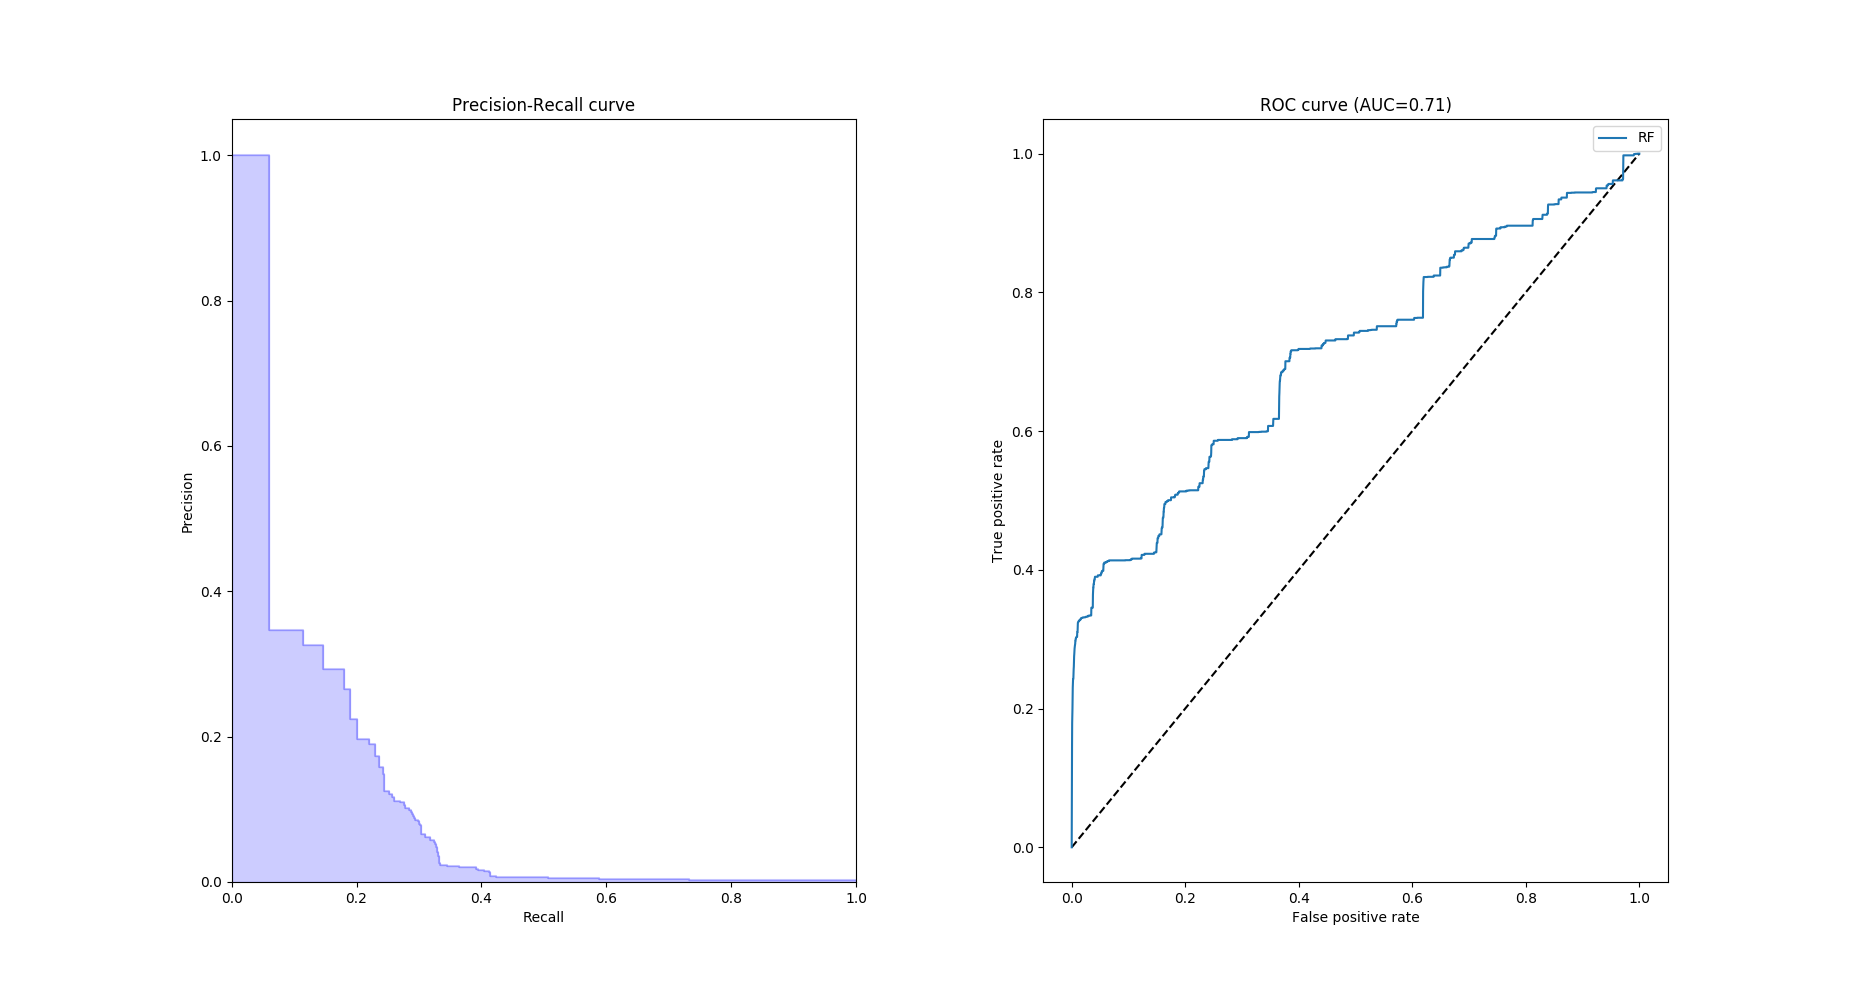
\includegraphics[width=\textwidth]{images/customAna-stem}
    \caption{Results Analyzer extended with Stemming}
    \label{fig:stemming}
\end{figure}

\subsubsection{$n$-grams}\label{sec:ngrams}
Now, let's see what happens if we divide the words into tuples of length $n$. This is called $n$-gram filtering\footnote{\texttt{org.apache.lucene.analysis.ngram.NGramTokenFilter}}. We tried 6 different values for $n = \{2, 3, 4, 5, 6, 8\}$.

For all $n$, the ROC curve is almost identical to the previous ones, but it's the PR curve that's giving an interesting result. In figure \ref{fig:ngram4}, you will find an example of such a plot (for $n = 4$). We have no idea if this result is due to how we've built our queries, or if it comes from the way we're using the data. Our best guess would be that $n$-grams are technically only interesting to use if you were to allow wildcards and the queries on which we test don't use them.

The empty plots you see are, in fact, PR-curves that have a precision close to 0, no matter the value for the recall.

It is clear we get better results without the usage of $n$-grams, which is why we will not include them in our optimizations.

\begin{figure}[htp]
    \centering
    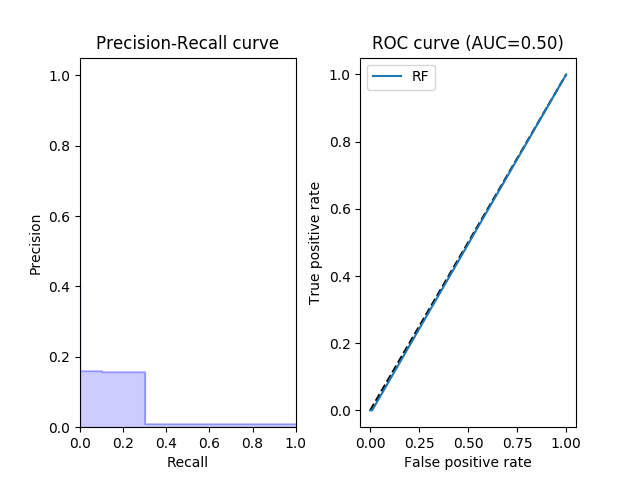
\includegraphics[width=\textwidth]{images/customAna-n4}
    \caption{An overview of the extended Analyzer for $n$-gram filtering, where $n = 4$.}
    \label{fig:ngram4}
\end{figure}

\subsection{Manual Thesaurus-Based Query Expansion}\label{sec:synonyms}
A thesaurus is a list of synonyms. For each term in our dictionary, we may create such a list to associate the words with. Theoretically, this should increase our general recall, but may decrease precision, especially when we're talking about homonyms and such.

As a last improvement, we create such a filter\footnote{\texttt{org.apache.lucene.analysis.synonym.SynonymFilter}} and add it to the analyzer. This way, for each word we see, a set of synonyms will be associated with it, using a \texttt{SynonymMap}\footnote{\texttt{org.apache.lucene.analysis.synonym.SynonymMap}}. Use used an offline dictionary of thesaurus, \cite{synonyms}, which is built with approximately $169\,000$ English words and is two-directional.

To our surprise there was a slight increase in performance (approximately 3\% in terms of AUC), meaning that the some synonyms were actually needed to score better. This is shown in figure \ref{fig:synonyms}.
\begin{figure}[htp]
	\centering
	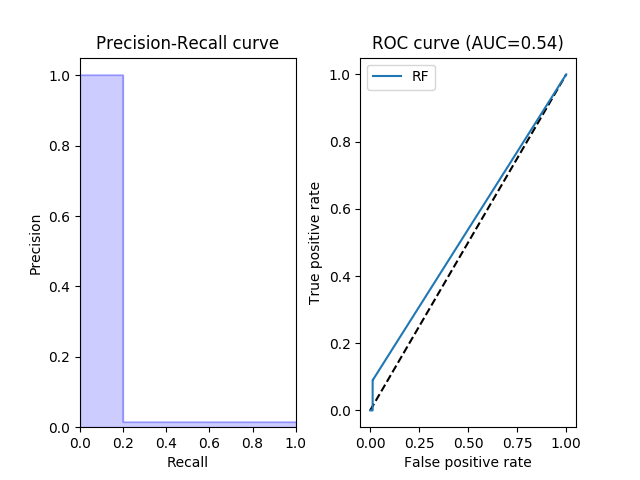
\includegraphics[width=\textwidth]{images/customAna-synonym}
	\caption{An overview of the extended Analyzer for manual thesaurus-based query expansion.}
	\label{fig:synonyms}
\end{figure}


\subsection{Final Results}
A final result of our benchmarking study can be found in figure \ref{fig:synonyms}, where everything comes together: lower case conversion, trimming, removing of non-alphanumeric values, word delimiters, stemming, and thesaurus-based manual query-expansion.

Note that $n$-grams are not included in this result.

\section{Rocchio Algorithm}\label{sec:rocchio}
Next, we wanted to apply the \textsf{Rocchio} algorithm for pseudo-relevance feedback. It's principle is simple: we search for a query, mark some documents as ``\textit{relevant}'' and change the angle of our query vector so it is located in the center of the cluster of relevant documents\footnote{Note that this method assumes all relevant documents are located in the same cluster.}.

Unfortunately, we hit a brick wall. And we hit it hard. In theory, there is no problem. We apply the Rocchio formula as given below to our original query $Q_o$:
$$\overrightarrow{Q_n} = \alpha \overrightarrow{Q_o} + \beta \frac{1}{|D_R|} \sum_{\overrightarrow{Q_j} \in D_R}{\overrightarrow{Q_j}} + \gamma \frac{1}{|D_{NR}|} \sum_{\overrightarrow{Q_k} \in D_{NR}}{\overrightarrow{Q_k}}$$
Let's ignore the scale factors $\alpha$, $\beta$ and $\gamma$ for now. In section \ref{sec:bstudy}, we described a way to easily and uniformly determine if a document was ``\textit{correct}'' (read: \textit{relevant}) or not. So we have a query $q$, a set of relevant documents $D_R$ and a set of irrelevant documents $D_{NR}$ (which can be obtained from the simple truth that $D_R + D_{NR} = D$, where $D$ represents the set of all documents). Because we remembered the frequency vectors (see section \ref{sec:fv}), we can easily transform all these variables into their corresponding vectors and apply the formula.

As you might recall, we described in the beginning of section \ref{sec:query} that Lucene does not work nicely with manipulating the VSM and searching by queries. Yet, we decided not to create a custom system for searching the documents, due to the sheer size of our data. This decision sort of came back to haunt us.

Because we did not develop such a system and thus do not have an optimized method for searching (and sorting) our documents, we have to map our custom feature vectors onto a Lucene boolean query string. Lucene's query syntax (found in \cite{lucene}) provides a way to add a \textit{boost} to each term in the query. Hence, for each term in our resulting query vector $\overrightarrow{Q_n}$, we give it a boost of its absolute value and negate it if the original value in $\overrightarrow{Q_n}$ was negative.

For instance, if $\overrightarrow{Q_n}$ states that the term ``\texttt{python}'' has a score of 5.6 and ``\texttt{abstract}'' has a score of -9.123, our resulting query string would be ``\texttt{python\string^5.6 -abstract\string^9.123}''.

Now, for each word in our vocabulary (which counts approximately $20\,000$ words), we have a term in our query string\footnote{Since we drop all terms that would have a \textit{boost} of 0, this is slightly less than our entire vocabulary, but the difference is nullable.}. Also, Lucene cannot handle boolean queries that count over $1\,024$ words (by default), so having almost 20 times that size is difficult.

We can solve this issue by saying that Lucene must ignore the maximal clause count as follows:
\begin{lstlisting}[language=Java]
BooleanQuery.setMaxClauseCount(Integer.MAX_VALUE);
\end{lstlisting}

In hindsight, Lucene put that number by default to $1\,024$ for a good reason. As soon as this value is exceeded, it takes notably longer\footnote{In fact, the process was sooner killed, due to ``hanging'' than it finishing for a single query.} to execute a simple search, so this is not the solution we were aiming for.

On top of that, notice how we must apply a mathematical formula to vectors of size $20\,000$. This formula takes an incredibly long time to compute, causing our benchmarking to be estimated to take 80 hours to run (if we were to limit the query generation to a mere 500 terms, which is a massive oversight in itself). And this is even ignoring the fact that we wanted to test it out for different values of $\alpha$, $\beta$ and $\gamma$.

Long story short, the way we have approached Rocchio is not the way to go. An optimization would be to set both $\beta$ and $\gamma$ to 0, but then we technically don't do anything. Another solution would be to limit our dataset to very few documents, but here the issues remain the same (with still an estimate of a couple of days).

Due to time constrains and the lacking documentation of Lucene on this front, we believe Rocchio (or other kinds of pseudo-relevance feedback) not to be possible with the current setup of our system.

\clearpage
\bibliographystyle{abbrv}
\bibliography{mybib}

\end{document}
